\documentclass[border=4pt]{standalone}
\usepackage[utf8]{inputenc}\usepackage[T1]{fontenc}\usepackage{mathptmx}
\usepackage{tikz}\usetikzlibrary{positioning,arrows.meta,calc}
\begin{document}
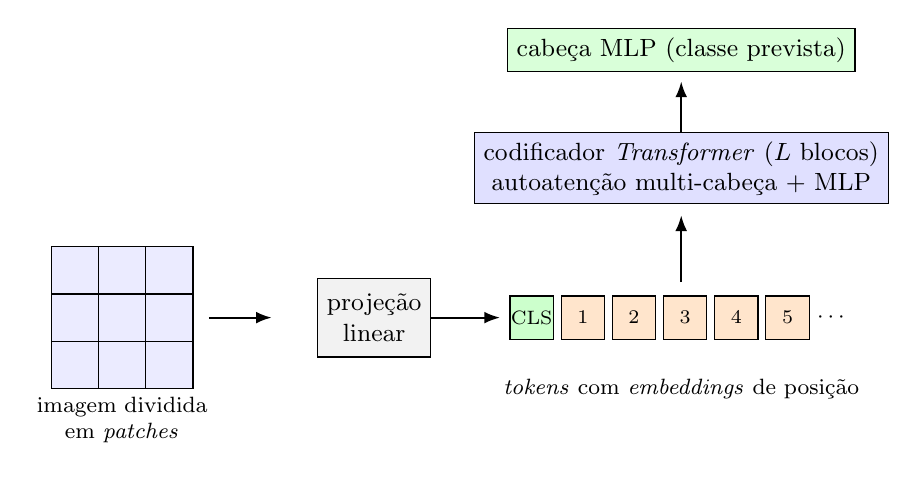
\begin{tikzpicture}[font=\small,arr/.style={-{Latex[length=2mm]},thick},
  tok/.style={draw,fill=orange!20,minimum width=0.55cm,minimum height=0.55cm,inner sep=0pt,font=\scriptsize}]
% image grid
\foreach \i in {0,1,2} \foreach \j in {0,1,2} \draw[fill=blue!8] (\i*0.6,-\j*0.6) rectangle ++(0.6,-0.6);
\node[align=center,font=\footnotesize] at (0.9,-2.2) {imagem dividida\\em \textit{patches}};
\draw[arr] (2.0,-0.9) -- (2.8,-0.9);
\node[draw,fill=gray!10,align=center,minimum height=1.0cm] (proj) at (4.1,-0.9) {projeção\\linear};
\draw[arr] (proj.east) -- (5.7,-0.9);
\node[tok,fill=green!20] (cls) at (6.1,-0.9) {CLS};
\foreach \k in {1,...,5} \node[tok] at (6.1+\k*0.65,-0.9) {\k};
\node[font=\footnotesize] at (9.9,-0.9) {$\cdots$};
\node[align=center,font=\footnotesize] at (8.0,-1.8) {\textit{tokens} com \textit{embeddings} de posição};
\draw[arr] (8.0,-0.45) -- (8.0,0.4);
\node[draw,fill=blue!12,minimum width=5.0cm,minimum height=0.9cm,align=center] (enc) at (8.0,1.0) {codificador \textit{Transformer} ($L$ blocos)\\autoatenção multi-cabeça + MLP};
\draw[arr] (enc.north) -- (8.0,2.1);
\node[draw,fill=green!15,align=center] at (8.0,2.5) {cabeça MLP (classe prevista)};
\end{tikzpicture}
\end{document}
